%% NOTES TO SELVES
%% ---------------
%% - This is the first paper that discusses how to be systematic about coordinate freedom in ML.
%% - HOGG: Carry the example of FINANCE through everything here, just to make sure we have non-physics examples everywhere. It has both coordinate and units considerations.
%% Adjust the description on how we got the magnitude of the missing constant in the black body problem.

\documentclass{article}
\usepackage{microtype}
\usepackage{graphicx}
% \usepackage{booktabs} % for professional tables

% hyperref makes hyperlinks in the resulting PDF.
% If your build breaks (sometimes temporarily if a hyperlink spans a page)
% please comment out the following usepackage line and replace
% \usepackage{icml2023} with \usepackage[nohyperref]{icml2023} above.
\usepackage{hyperref}

% Attempt to make hyperref and algorithmic work together better:
\newcommand{\theHalgorithm}{\arabic{algorithm}}

% Use the following line for the initial blind version submitted for review:
% \usepackage{icml2023}
% If ACCEPTED, instead use the following line for the camera-ready submission:
% \usepackage[accepted]{icml2023}
% For ARXIV, but BEFORE acceptance, uncomment the following two lines (AND UNCOMMENT THE ACKS):
\usepackage[accepted]{icml2023}
\makeatletter\renewcommand{\ICML@appearing}{Copyright 2023 the authors.}\makeatother

% For theorems and such
\usepackage{amsmath}
\usepackage{amssymb}
\usepackage{mathtools}
\usepackage{amsthm}

% if you use cleveref..
% \usepackage[capitalize,noabbrev]{cleveref}

%%%%%%%%%%%%%%%%%%%%%%%%%%%%%%%%
% THEOREMS
%%%%%%%%%%%%%%%%%%%%%%%%%%%%%%%%
\theoremstyle{plain}
\newtheorem{theorem}{Theorem}[section]
\newtheorem{proposition}[theorem]{Proposition}
\newtheorem{lemma}[theorem]{Lemma}
\newtheorem{corollary}[theorem]{Corollary}
\theoremstyle{definition}
\newtheorem{definition}[theorem]{Definition}
\newtheorem{assumption}[theorem]{Assumption}
\theoremstyle{remark}
\newtheorem{remark}[theorem]{Remark}
\newtheorem{principle}[theorem]{Principle}

% Todonotes is useful during development; simply uncomment the next line
%    and comment out the line below the next line to turn off comments
%\usepackage[disable,textsize=tiny]{todonotes}
\usepackage[textsize=tiny]{todonotes}

% add our our own custom macros
\usepackage{amsmath}
\usepackage{amssymb}
\usepackage{tikz-cd}
\tikzcdset{every label/.append style = {font = \normalsize}}
\newcommand{\documentname}{\textsl{Article}}
\newcommand{\sectionname}{Section}
\newcommand{\secref}[1]{\sectionname~\ref{#1}}
\newcommand{\figref}[1]{Figure~\ref{#1}}
\newcommand{\bernhard}[1]{ \textcolor{red}{\textbf{~B: #1}}}
\newcommand{\soledad}[1]{ \textcolor{blue}{\textbf{~S: #1}}}
\newcommand{\inv}{^{-1}}
\newcommand{\T}{^\top}
\newcommand{\R}{{\mathbb R}}
\newcommand{\surf}{{\mathrm{s}}}
\newcommand{\unit}[1]{\mathrm{#1}}
\newcommand{\kg}{\unit{kg}}
\newcommand{\m}{\unit{m}}
\newcommand{\s}{\unit{s}}
\newcommand{\K}{\unit{K}}

% The \icmltitle you define below is probably too long as a header.
% Therefore, a short form for the running title is supplied here:
\icmltitlerunning{~ \hfill The passive symmetries of machine learning \hfill \thepage}
\frenchspacing\sloppy\sloppypar\raggedbottom
\begin{document}

\twocolumn[
\icmltitle{The passive symmetries of machine learning
%Towards covariant machine learning
%Passive symmetries make every machine learning problem equivariant
}

\icmlsetsymbol{equal}{*}

\begin{icmlauthorlist}
\icmlauthor{Soledad Villar}{equal,JHU,MINDS}
\icmlauthor{David W. Hogg}{equal,CCPP,MPIA,Flatiron}
\icmlauthor{Weichi Yao}{Stern}
\icmlauthor{George A. Kevrekidis}{JHU,LANL}
\icmlauthor{Bernhard Sch\"olkopf}{MPI-IS}
\end{icmlauthorlist}

\icmlaffiliation{JHU}{Department of Applied Mathematics and Statistics, Johns Hopkins University, Baltimore MD, USA}
\icmlaffiliation{MINDS}{Mathematical Institute for Data Science, Johns Hopkins University, Baltimore MD, USA}
\icmlaffiliation{CCPP}{Center for Cosmology and Particle Physics, Department of Physics, New York University, New York NY, USA}
\icmlaffiliation{MPIA}{Max-Planck-Insitut f\"ur Astronomie, Heideilberg, Germany}
\icmlaffiliation{Flatiron}{Flatiron Institute, a division of the Simons Foundation, New York NY, USA}
\icmlaffiliation{Stern}{Department of Technology, Operations, and Statistics, Stern School of Business, New York University, New York NY, USA}
\icmlaffiliation{LANL}{Los Alamos National Laboratory, Los Alamos NM, USA}
\icmlaffiliation{MPI-IS}{Max Planck Institute for Intelligent Systems, T\"ubingen, Germany}

\icmlcorrespondingauthor{David W. Hogg}{david.hogg@nyu.edu}

% You may provide any keywords that you
% find helpful for describing your paper; these are used to populate
% the "keywords" metadata in the PDF but will not be shown in the document
\icmlkeywords{symmetry, equivariance, physics, group theory}

\vskip 0.3in
]

% this must go after the closing bracket ] following \twocolumn[ ...

% This command actually creates the footnote in the first column
% listing the affiliations and the copyright notice.
% The command takes one argument, which is text to display at the start of the footnote.
% The \icmlEqualContribution command is standard text for equal contribution.
% Remove it (just {}) if you do not need this facility.

%\printAffiliationsAndNotice{}  % leave blank if no need to mention equal contribution
\printAffiliationsAndNotice{\icmlEqualContribution} % otherwise use the standard text.

\begin{abstract}
%This purely conceptual paper extends the applicability of group-equivariant methods in machine learning to almost all of ML.
Any representation of data involves arbitrary investigator choices.
Because those choices are external to the data-generating process, each choice leads to an exact symmetry, corresponding to the group of transformations that takes one possible representation to another.
These are the \emph{passive symmetries}; they include coordinate freedom, gauge symmetry and units covariance, all of which have led to important results in physics.
Our goal is to understand the implications of passive symmetries for machine learning: Which passive symmetries play a role (e.g., permutation symmetry in graph neural networks)? What are \emph{dos and don'ts} in machine learning practice?
We assay conditions under which passive symmetries can be implemented as group equivariances.
We also discuss links to causal modeling, and argue that 
the implementation of passive symmetries is particularly valuable when the goal of the learning problem is to generalize out of sample.
While this paper is purely conceptual, we believe that it can have a significant impact on helping machine learning make the transition that took place for modern physics in the first half of the Twentieth century.
\end{abstract}

\section{Introduction}\label{sec:intro}

Many important ideas in machine learning (ML) have come from---or been inspired by---mathematical physics.
These include the kernel trick \cite{CouHil53,SchSmo02} and the use of statistical mechanics techniques to solve probabilistic problems \cite{mcmc, gibbs}.
Here we suggest another connection between physics and ML, which relates to representation of observables:
When features and labels are represented in a mathematical form that involves investigator choices, the ML method (or any relevant function) ought to be written in a form that is exactly equivariant to changes in those investigator choices.
These ideas appear in the physics literature as early as \citet{gr}. They are given in the introduction of \textit{The Classical Groups} by \citet{weyl} as a motivation to study group theory.
The first sentences of \textit{Modern Classical Physics} by \citet{mcp} say
\vspace{-1.5ex}\begin{quote}
[...] a central theme will be a Geometric Principle: 
The laws of physics must all
be expressible as geometric (coordinate-independent and reference-frame-independent)
relationships between geometric objects (scalars, vectors, tensors, ...) that represent
physical entities.
\end{quote}\vspace{-1.5ex}
This principle leads to the important physical symmetries of coordinate freedom and gauge symmetry; a small generalization would include units covariance.
Each of these symmetries has led to fundamental results in physics. Some of these ideas are also exploited in ML, in particular in the geometric deep learning literature \cite{bronstein2021geometric, weiler}. 
We argue---in this purely conceptual contribution---that analogs of these symmetries could have big impacts in ML, and enormously increase the scope of group-equivariant methods in ML.

In natural science there are two types of symmetries (see, for example, Section 4.1 of \citealt{rovelli2000loop}). 
The first kind is \emph{passive}, arising from the arbitrariness of the mathematical representation described above.
An example familiar to machine learners is the equivariance of functions on graphs to the relabeling of the graph nodes.
This is an exact, passive symmetry; graph neural network architectures (GNNs) build this passive symmetry in by design \cite{bruna2013spectral, duvenaud2015convolutional, gilmer2017neural}. 
An example familiar to physicists is what we call \emph{units covariance}, which is the requirement that any correct description of the world have inputs and outputs with the correct units.
This passive symmetry leads to remarkable results; we discuss these in \secref{sec:units}.

The second kind of symmetries is {\em active}.
These are the ones that must be established by observations and experiments.
The fundamental laws of physics do not seem (at current precision) to depend on position, orientation, or time, which in turn imply conservation of momentum, angular momentum and energy (the celebrated theorem of \citealt{noether}).
Of course the motion of a particle depends on time and position! But the fundamental laws governing the motion don't themselves appear to depend on the absolute value of the time, nor the position of the experimental apparatus.
Active symmetries like these are empirical and can be falsified by experimental tests.
Both active and passive symmetries can be expressed in terms of group or groupoid actions and equivariances, but their epistemological content and range of applicability are very different. 

In this contribution, we argue that passive symmetries apply to essentially all data analysis problems.
They have implications for how we structure ML methods. While we provide some examples, most of our contributions are conceptual:

\textbf{Our contributions:}
\vspace{-1.5ex}\begin{itemize}
\itemsep 0.5\parskip
\topsep 0pt
\partopsep 0pt
\parskip 0pt
\item
We introduce the concept of passive symmetries to ML.
While this is an old concept in classical physics, it has not been applied widely in ML.
\item
We give a formal definition of passive symmetries in terms of group actions and explain how passive symmetries are always in play in data problems.
\item
We illustrate with toy examples how enforcing passive symmetries can improve regressions. 
\item
We demonstrate that imposing passive symmetries can lead to the discovery of important hidden objects in a data problem.
\item
We draw connections with causal inference.
One is that all causal graphs and mechanistic models are constrained to be consistent with the passive symmetries.
Another is that the determination that a data problem has all the inputs necessary to express the symmetry exactly looks like a causal inference.
\item 
We provide guidance on how to structure ML models so that they respect the passive symmetries. We call out some current standard practices that prevent models from obeying symmetries. 
% \item
% We provide a glossary that can be used to translate ideas between physics and ML. 
\end{itemize}\vspace{-1.5ex}
Some of the ideas seem deceptively simple, yet they have profound implications. Since ML has not yet absorbed these notions as naturally as physics has, we need to discuss analogies to physics in some detail. We have tried to make the discussion accessible to an ML audience; the Appendices includes a glossary that can be used to translate ideas between physics and ML.

\section{Passive symmetries}\label{sec:informal}

\begin{figure}
    \centering
    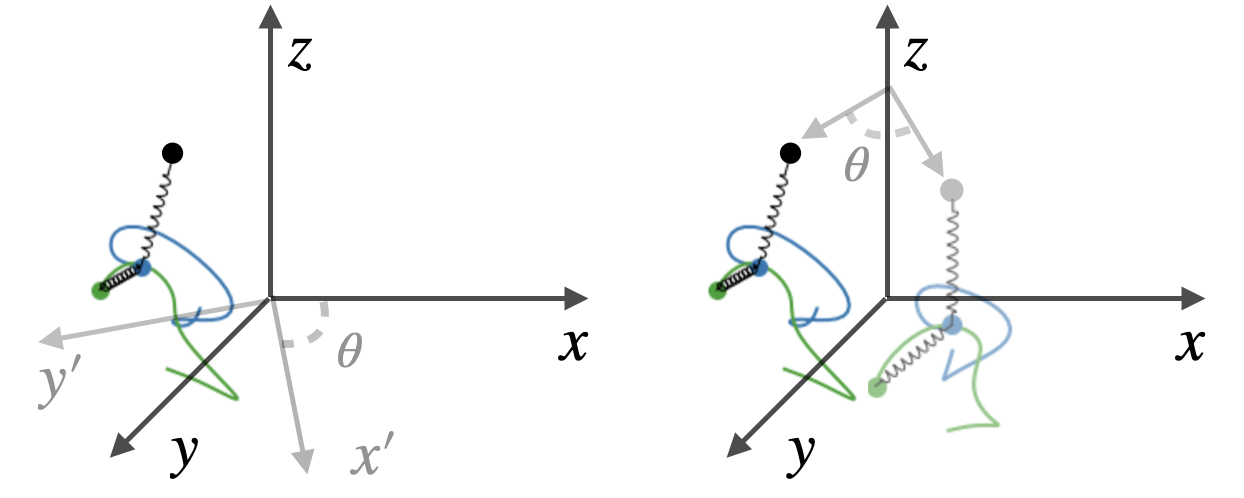
\includegraphics[width=0.45\textwidth]{alias.png}
    \vspace{-1.5ex}
    \caption{Figure depicting the difference between active and passive transformations. \textsl{(Left panel)}: The passive or alias transformation corresponding to a rotation of the coordinates through an angle $\theta$ in the xy-plane. The equivariance of the dynamics with respect to this tranformation is a passive symmetry. \textsl{(Right panel)}: The active or alibi transformation corresponding to a rotation of the double pendulum state through an angle $-\theta$ in the xy-plane. Equivariance with respect to this transformation is an active symmetry.}
    \vspace{-2.5ex}
    \label{fig:alias}
\end{figure}

Passive symmetries arise from redundancies or free parameters or investigator choices in the representation of data.
They are to be contrasted with the active symmetries, which arise from observed or empirical invariances of the laws of physics with respect to parameters, like position, velocity, particle labeling, or angle.
Passive symmetries can be established with no need of observations, as they arise solely from the principle that the physical world is independent of the mathematical choices we make to describe it.
The groups involved in coordinate freedom can be large and complicated (for example, groups of reparameterizations).

A big part of the literature on equivariant ML is implicitly or explicitly looking at \emph{active} symmetries.
This is possibly because in most problems the coordinate system is fixed before the problem is posed, and both training and test data are expressed in those fixed coordinates.
If a data set is made with a fixed coordinate system, but still exhibits an {\em observable} invariance or equivariance with respect to (say) rotations, then that represents an active symmetry.
However, cases of exact active symmetries are rare; they only really appear in natural-science contexts like protein folding or cosmology.
For example, in a protein folding problem, the way the protein folds may not depend on its orientation in space (rendering the problem actively O(3) equivariant).
This finding relies on the (empirical) observation that the local gravitational field (on Earth) does not affect the folding.
This may be approximately true or assumed or experimentally established; it is an active symmetry.
In contrast, the fact that the protein folds in a way that doesn't depend on the coordinate system chosen to describe it is absolutely and always true; it is not experimentally established; it is a passive symmetry.

The relationship between active and passive symmetries is reflected in the relationship between what are sometimes called active and passive transformations, or \emph{alibi} and \emph{alias} transformations, depicted in Figure \ref{fig:alias}.
An active or alibi transformation is one in which the objects of study are moved (rotated, translated, interchanged, etc.).
A passive or alias transformation is one in which the coordinate system in which the objects of study are described is changed (rotated, translated, relabeled, etc.).
Mathematically, the two kinds of transformations seem very similar:
For example, how do we know whether we rotated all the vectors in our problem by $30\,\deg$, or else rotated the coordinate system used by $-30\,\deg$?
The answer is that if you rotated \emph{absolutely all} the vectors (and tensors) in your problem, including possibly many latent physical vectors, then there would be no mathematical difference.
But in real problems, where some vectors can't be actively rotated (think, for example of the local gravitational-field vector, or the vector pointing towards the Sun), or some may not be known or measurable, the two kinds of transformations are different.

The protein-folding example suggests that it is hard to implement or enforce a true passive symmetry in a real data-analysis problem.
It requires us to incorporate all relevant contextual information.
How do we know if all relevant features are part of our data set?
We could perform the protein-folding experiment in a closed, isolated environment to make sure no external forces are in play;
this is impossible for many practical applications, and furthermore there could still exist fundamental constants that are not part of our model or knowledge (see \secref{sec:experiments}).
Another approach is to perform the experiment multiple times after actively putting the molecules into different orientations.
If the protein folds differently, we learn that the problem is not symmetric with respect to the 3d coordinates of the molecule, and therefore when a rotation is performed there must be at least one more vector that needs to be rotated as well (for instance, the gravity vector or the eigenvectors of a stress tensor, say).
This identification of all necessary inputs to establish the passive symmetry is similar to the problem of performing interventions to learn the existence of confounding factors in causal inference.
We will come back to the connections to causality in \secref{sec:causality}.

Once a passive symmetry---and all relevant contextual information---is identified, we want to write the data analysis problem or learned function such that it is exactly \emph{equivariant} with respect to the relevant group:
If the representation or coordinate system of the inputs is changed, the representation or coordinate system of the output should change correspondingly.
ML methods that are not constrained to respect passive symmetries are doomed to make certain kinds of mistakes.
We will provide some examples thereof in \secref{sec:dos}.

The most restrictive form of the Geometric Principle quoted in \secref{sec:intro} states that physical law must be written in terms of vectors, tensors, and coordinate-invariant scalars.
These objects can only be combined by rules set out in the Ricci calculus (\citealt{ricci}; sometimes Einstein summation notation, \citealt{einstein}).
This calculus was introduced to make objects equivariant to coordinate diffeomorphisms on curved manifolds.
In the Ricci calculus, objects are written in index notation (a scalar has no indices, a vector has one index, and a $k$-tensor has $k$ indices), outer products are formed, and only certain kinds of sums over pairs of indices are permitted.
When the inputs to a function are scalars, vectors, and tensors, and the function conforms to the rules of the Ricci calculus, the function will produce a geometric output (a scalar, vector, or tensor,\footnote{%
It should be noted here that with the word ``vector'' and ``tensor'' here we are making specific technical reference to true vectors and tensors in 3-space, subject to passive $O(3)$ symmetries, like (physical) velocities, accelerations, and stress tensors.
We are \emph{not} including arbitrary lists or tables of data or coefficients, which are sometimes called ``vectors'' and ``tensors'' in ML contexts.}
depending on the number of unsummed indices), and the function will be precisely equivariant to rotations and reflections of the coordinate system.
This is how a large class of passive symmetries are enforced in physics contexts.

There are many other passive symmetries, including coordinate diffeomorphisms, reparameterizations (including canonical transformations), units covariance (see \secref{sec:units}), and gauge.
Some of these are easy to implement and some are difficult;
not all passive symmetries have practical implementations available at present.

The passive coordinate diffeomorphism symmetry on curved manifolds has been tremendously important in the development of contemporary physics.
Einstein, for example, found the equations of general relativity by looking at every expression to some polynomial degree consistent with the passive symmetry enforced by the Ricci calculus (he called this family of polynomials \emph{covariant}\footnote{Following the lead of physics, we could in principle call ML methods equivariant to passive symmetries ``covariant''.}
) until he found the one that reduced to Newtonian gravity in the weak-field limit \cite{gr}. Even before that, while not expressed in terms of passive symmetry, the discovery of special relativity \cite{sr} can be thought of as the decision to move an active symmetry (the observation that the speed of light is the same for all observers) into a passive symmetry (Lorentz invariance). We stress that these insights were truly profound \cite{EARMAN1978251}; they revolutionized physics; not too long before Einstein, such considerations would have been highly unusual. 
Similarly, passive symmetries do not feature in today's ML practice---if the development of physics is any indication, their potential could be very significant.

\section{Example: Units covariance}\label{sec:units}

Perhaps the most universal passive symmetry is units covariance---the behavior of a system doesn't depend on the units system in which we write the measured quantities.
It is a passive symmetry with extremely useful consequences.

Consider a mass $m$ near the surface of the Earth, close enough to the surface such that the gravitational field can be considered to be determined by a constant (not spatially varying) vector with magnitude $g$ and direction downwards.
\textsl{Question~1:}~If this mass $m$ is dropped (released at rest) from a height $h$ from above the ground, how much time $T$ does it take to fall to the ground?
\textsl{Question~2:}~If this mass $m$ is launched from the surface at a velocity of magnitude $v$ at an angle $\theta$ to the horizontal, how much horizontal distance $L$ will it fly before it hits the surface again?
Assume that only $m, g, h$ come in to the solution;\footnote{We will return to this seemingly innocuous point below.} assume that the height $h$ and the velocity $v$ are both small enough that air resistance, say, can be ignored.

The answers to these questions are almost completely determined by dimensional (or units-covariance) arguments.
The mass $m$ has units of $\kg$, the gravitational acceleration magnitude $g$ has units of $\m\,\s^{-2}$, the velocity magnitude $v$ has units of $\m\,\s^{-1}$, the time $T$ has units of $\s$, and the lengths $h$ and $L$ have units of $\m$.
The angle $\theta$ is dimensionless.
The only possible combination of $m, g, h$ that has units of time is $\alpha\,\sqrt{h/g}$, where $\alpha$ is a dimensionless constant, which doesn't depend on any of the inputs.
The only possible combination of $m, g, v, \theta$ that has units of length is $\beta(\theta)\,v^2/g$, where $\beta(\theta)$ is a dimensionless function of only one dimensionless input.
That is, both Questions~1 and 2 can be answered up to a dimensionless prefactor without any considerations beyond those of the units of the inputs and outputs, and without any training data.
And both of those answers don't depend in any way on the input mass $m$, which is a fundamental observation \cite{gr}.

This shows that a function can sometimes be inferred from units covariance only, i.e., from a purely passive symmetry.
Units covariance has been introduced to ML methods previously \cite{villar2022dimensionless, bakarji2022dimensionally, xie2022data}.
It can help with training, predictive accuracy, and out-of-sample generalization.
In particular, out-of-sample generalization improves because the enforcement of the symmetry enforces scaling properties of the learned function.
These, in turn, help make predictions when the test data are outside the range of the training data.

\section{Formal definition}\label{sec:definitions}

Consider $\mathcal X$ to be the state space of a specific physical system (for instance $x\in \mathcal X$ could be the positions, velocities, masses, spins, and charges of a set of particles at a given time). 
We consider a family of maps $\{\Phi_i: \mathcal X \to \mathcal H_i\}_{i\in \mathcal I}$ where the $\mathcal H_i$ are spaces of observations or encodings indexed by $i\in \mathcal I$ (for instance $\Phi_i(x)$ could be the total mechanical energy of the system $x$ at a set of times measured in joules, and $\Phi_j(x)$ could be in kcal, etc).
The family of maps $\{\Phi_i\}_{i\in \mathcal I}$ not only describes the possible observables but also a way to express those observables in a specific coordinate system and with specific units. 

We say that two encodings $\Phi_i$ and $\Phi_j$ are compatible if there exists an invertible morphism $\beta_{j}^i:\Phi_i(\mathcal X)\to  \Phi_j(\mathcal X)$ that makes the diagram \eqref{eq.diagram} commute.
\vspace{-1.5ex}
\begin{equation}\label{eq.diagram}
\small
\begin{tikzcd}[every label/.append style = {font = \small}]
  {\cal X}\arrow[r,"id"] \arrow[d,"\Phi_i",swap] & {\cal X}  \arrow[d,"\Phi_j"]\\
{\mathcal H_i} \arrow[r,"\beta_{j}^i"]  & {\mathcal H_j} 
\end{tikzcd}
\vspace{-1.5ex}
\end{equation}
Note that not all observables are compatible. We expect that observables of different types (for instance, masses and positions) are not compatible. Which observables are compatible depend on the definition of the spaces $\mathcal H_i$ and the invertible morphisms $\beta$ between them.
%Namely, the encodings $\Phi_i$ and $\Phi_j$ are compatible (or \emph{equivalent}) if they express the same aspect of the world in possibly different representation. WE SHOULD FURTHER DISCUSS THIS POINT. For instance in under this definition if $\Phi_i(x)$ is the p 

The passive symmetries are the groupoid of invertible morphisms $\beta$ between compatible encodings that make the diagram commute $\mathcal P = \{\beta: \Phi_i(\mathcal X) \to \Phi_j(\mathcal X) \text{ s.t. } \beta\circ \Phi_i = \Phi_j, \, i,j\in \mathcal I \}$, where the groupoid operator is the composition. We note that this is a groupoid and not a group because not every pair of transformations are composable. 
The groupoid of passive symmetries $\mathcal P$ consists of all the possible changes of coordinates or automorphisms between encodings or observables. 

Critical to the definition is that we establish beforehand the spaces of possible observables or encodings $\mathcal H_i$, the observables or encodings $\Phi_i$; and the class of invertible morphisms $\beta$. For instance, $\mathcal H_i$ can be in the category of smooth manifolds with smooth diffeomorphisms, or in the category of vector spaces with invertible linear transformations, or orthogonal transformations.   

For example, take $\mathcal X$ to be a protein. Each map $\Phi_i$ could encode a list of positions of each of its atoms in some coordinate system. The passive symmetries include reordering of the atoms, and changes of the coordinate system by any invertible morphism. We may restrict $\mathcal H_i$ to the category of smooth manifolds where the $\beta$'s are diffeomorphisms, or we may only allow the $\beta$'s to be orthogonal transformations that fix the origin. Restricting the space of valid coordinates naturally restricts the valid changes of coordinates and therefore the space of passive symmetries.

Active symmetries, on the other hand, can be thought as transformations of the world that preserve an observable property.
%Given a compatible family of encodings $\{\Phi_i\}_{i\in I}$ as above, we could say that a map $\alpha:\mathcal X \to \mathcal X$ represents an active symmetry if there exist $i,j\in I$ such that $\mathcal H_i = \mathcal H_j$ and the diagram \eqref{eq.diagram2} commutes. 
%\begin{equation}\label{eq.diagram2}
%\small
%\begin{tikzcd}[every label/.append style = {font = \small}]
%  {\cal X}\arrow[r,"\alpha"] \arrow[d,"\Phi_i",swap] & {\cal X}  \arrow[d,"\Phi_j"]\\
%{\mathcal H} \arrow[r,"id"]  & {\mathcal H} 
%\end{tikzcd}
%\end{equation}
They involve interventions in the physical system, and therefore they are typically empirical and approximate.
Not every passive symmetry corresponds to an active symmetry, nor vice versa.
%For instance there are passive symmetries that would translate into active symmetries w transformations of the world that are not physically possible (such as changing $g$).
%There are  alternative definitions of active symmetries that do not rely on observables. 

Imposing a passive symmetry on the structure of an ML model can permit the discovery of scalings, structures, or missing elements in the physical description of, or predictions about, the problem.
We illustrate these ideas with some toy examples below.
The passive symmetries are seemingly trivial statements about the world, but they lead to strong constraints on the laws of physics, and deliver scaling arguments that solve real problems in physics.
They can also constrain ML in valuable ways.
\emph{We conjecture that enforcing passive symmetries in ML and data-analysis tasks will lead to generalization improvements in a wide range of circumstances.}
In particular, we make this conjecture even for problems in which no (or few) active symmetries are present.
After all, most problems (like reading handwriting or predicting gravitational trajectories near the surface of the Earth) are not equivariant to rotations, reflections, and translations, but they are all, in their data-generating processes, exactly coordinate free, and exactly agnostic to the choices made in data representation.

\section{Experiments and examples}\label{sec:experiments}
\begin{figure*}[t!]
    \centering
    \begin{minipage}{0.45\textwidth}
    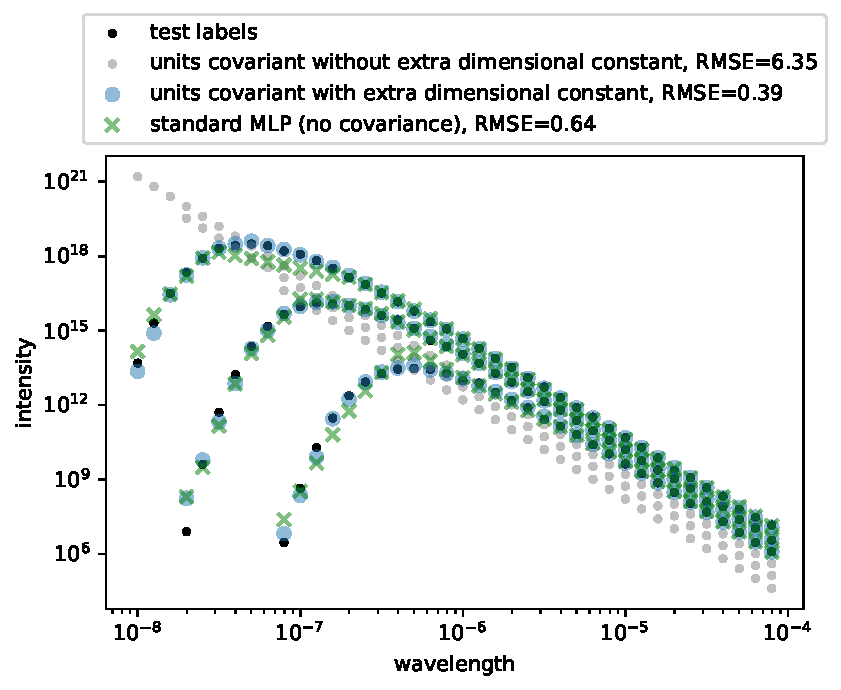
\includegraphics[height=0.85\textwidth]{units}
    \end{minipage}
    \begin{minipage}{0.5\textwidth}
    \centering
    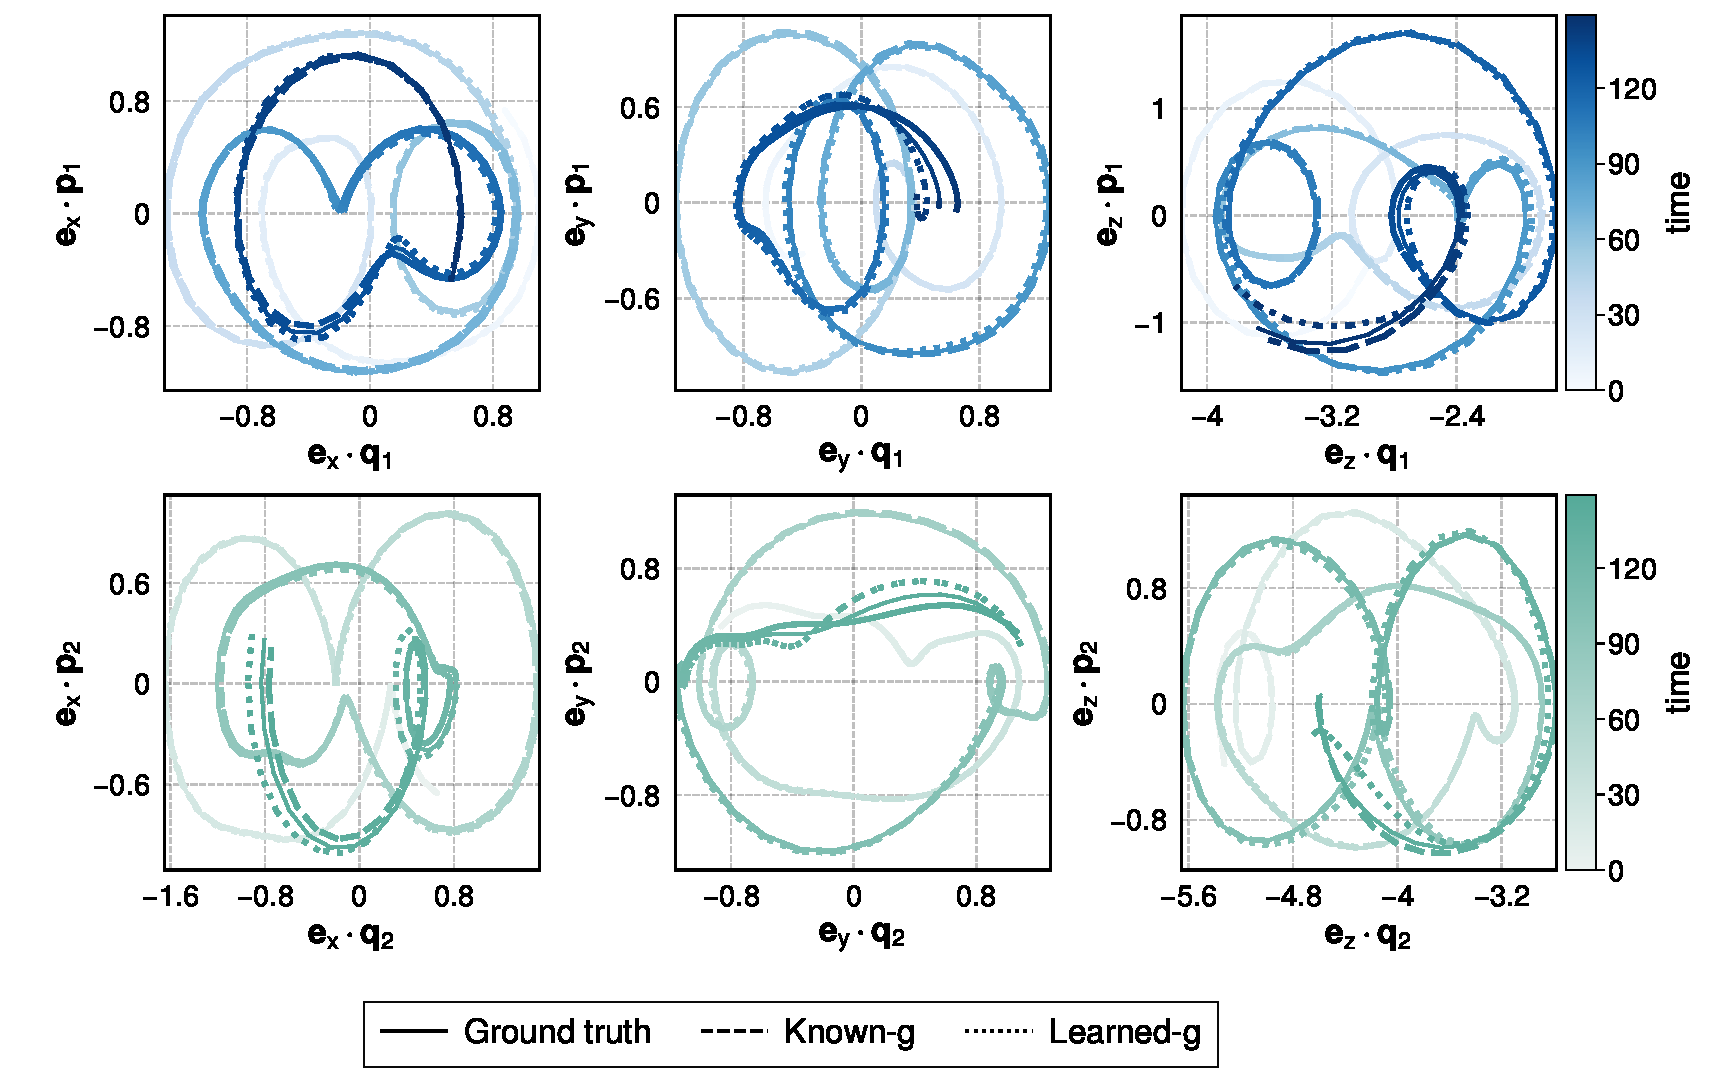
\includegraphics[width=0.99\textwidth]{pendulum}
    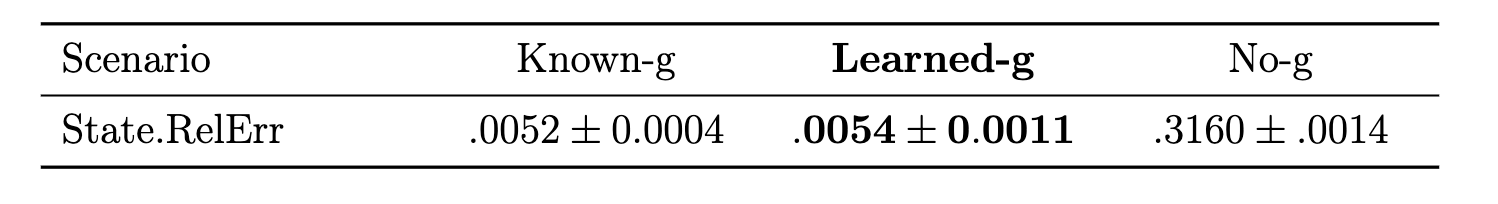
\includegraphics[width=0.99\textwidth]{table}
    \end{minipage}\vspace{-1.5ex}
    \caption{\textsl{(Left panel)}~We predict the intensity of black body radiation as a function of wavelength and temperature. For all experiments we use an MLP consisting of 3 layers with 20 hidden units each. The \emph{standard MLP} uses wavelength and temperature as features and it doesn't require the output to be dimensionally correct. The \emph{units covariant without extra constant} learns a scaling of the only dimensionally correct object one can construct with inputs $\lambda, T, c, k$ (see description main in text). The \emph{units covariant with extra dimensional constant} incorporates a constant with units $[\kg, \m, \s, \K]\in[-1,0,1]^4$ as an input feature, it performs a units covariant regression with the original features $\lambda, T, c, k$ and the extra constant. It then selects a constant with low validation error and reports the results on the test set. The constant learned for the depicted plot is 1.61e52 $\kg^{-1}\m^{-1}\s^{-1}\K^{-1}$, which is the same units and similar magnitude to the valid physical combination $c\,k\,h^{-2}$.
    \textsl{(Right panel)}~Performance of learning the dynamics of the springy double pendulum. We consider the three models (described in main text): (Known-g) an $O(3)$-equivariant model where the gravity is an input to the model, (No-g) an $O(3)$-equivariant model where the gravity is not given, and (learned-g) an $O(3)$-equivariant model that uses the position and momenta as well as an unknown vector that the model learns. The results show that $O(3)$-equivariance permits the learning of the gravity vector from data with only minimal impact in performance. See Appendix \ref{app:pendulum} for a more detailed description of the experiment.}
    \label{fig:my_label}
    \vspace{-1.5ex}
\end{figure*}

\textbf{Black-body radiation:}
An important moment in the history of physics was the discovery that the electromagnetic radiation intensity $B_\lambda$ (energy per time per area per solid angle per wavelength) of thermal black-body radiation can be described with a simple equation \cite{planck}
\begin{equation} \label{eq.planck}
    B_\lambda(\lambda) = \frac{2\,h\,c^2}{\lambda^5}\,\frac{1}{\exp\frac{h\,c}{\lambda\,k\,T} - 1}~,
\end{equation}
where $h$ is Planck's constant,
$c$ is the speed of light,
$\lambda$ is the wavelength of the electromagnetic radiation,
$k$ is Boltzmann's constant,
and $T$ is the temperature.
In finding this formula, Planck had to posit the existence (and units) of the constant $h=6.62607015\times 10^{-34}\,\kg\,\m^2\,\s^{-1}$ (Planck's original value was presented in $\mathrm{erg}\,\s$, which are different units but the same dimensions).
Prior to the introduction of $h$, the only dimensionally acceptable expression for the black-body radiation intensity was $B_\lambda(\lambda)=2\,c\,k\,T/\lambda^4$, which is the long-wavelength (infrared) or high-temperature limit.
Planck's discovery solved the ``ultraviolet catastrophe'' of classical physics.
This is the problem that, classically, the black-body spectrum, or any thermal object, ought to contain infinite numbers of excited modes at short wavelengths, or high frequencies, and thus infinite energy density.
Planck's solution seeded the development of quantum mechanics, which governs the behavior of all matter at small scales, and which cuts off the ultraviolet modes through quantization of energy.

Planck's problem can be solved almost directly with the passive symmetry of units covariance.
That is, the exponential cut-off of the intensity appears at a wavelength set by the temperature and a new constant, that must have units of action (or action times $c$, or action divided by $k$, or one equivalent in terms of the lattice of dimensional features, see \citealt{villar2022dimensionless}).

In \figref{fig:my_label} (left) we perform the following toy experiment:
We generate noisy samples of intensities as a function of wavelength and temperature according to \eqref{eq.planck}, and the learning task is to predict the intensity for different values of wavelengths and temperatures.
We perform a units covariant regression (employing the approach of \citealt{villar2022dimensionless}) using only $\lambda, T, c, k$; a units covariant regression with an extra dimensional constant found by cross-validation; and a standard MLP with no units constraints.
Our results show that no units-covariant regression for the intensity as a function of $\lambda, T, c, k$ can reproduce accurately the intensity $B_\lambda$. However when the regression is permitted to introduce a new dimensional constant (and remains units covariant given the new constant), it finds a constant with units (and, less precisely, magnitude) that is consistent with $h$ (or $h$ times a combination of $c$ and $k$). The units covariant model outperforms the baseline MLP. Again, this shows that the passive symmetry leads to powerful capability.

\textbf{Springy double pendulum:}
The double pendulum connected by springs is a toy example often used in equivariant ML demonstrations \cite{finzi2021practical,yao2021simple, villar2022dimensionless}. 
The final conditions (position and velocities of both masses after elapsed time $T$) are related to the initial conditions (position and velocities of the masses at the initial time), and the dynamics is classically chaotic.

The system is subject to a passive $O(3)$ symmetry (equivariance with respect to orthogonal coordinate transformations), and an active $O(2)$ symmetry (equivariance with respect to rotations and reflections in the 2-d plane normal to the gravity). 
The $O(3)$ symmetry is passive, because it is guaranteed by the fact that all vectors must be described in a coordinate system; nothing physical can change as the vectors undergo passive transformations because of coordinate-system changes.
The $O(2)$ symmetry is active, because it is an experimental fact that if the initial conditions are changed by an active or alibi rotation in the plane perpendicular to gravity, the dynamics and final state rotate accordingly.
Here we can see that the $O(2)$ active symmetry corresponds to the set of transformations in $O(3)$ that fix the gravity vector. 
%\bernhard{I think this needs more explanation, or ideally a picture that shows what are the coordinates. ML people won't get it otherwise.}

The $O(3)$ passive symmetry requires that the coordinates of all relevant vectors are transformed identically, the positions and momenta of both masses and the gravity vector. If the model doesn't contain all relevant vectors as inputs then the predictions will not be $O(3)$ equivariant. We perform an experiment in which we predict the dynamics of the double pendulum using $O(3)$-equivariant models. The symmetries are implemented by converting the network inputs (scalars and components of vectors) into invariant scalar quantities according to the Ricci calculus (which explicitly encodes $O(3)$), building the model in the space of the invariant scalars (as per \citealt{villar2021scalars}). The models implemented are \textsl{(Known-g)}---an $O(3)$-equivariant model that has the positions, momenta and gravity vector all as features (similar to the models in \citealt{villar2021scalars, yao2021simple}); \textsl{(No-g)}---an $O(3)$-equivariant model that that is missing the gravity vector as an input feature; and \textsl{(Learned-g)}\---an $O(3)$-equivariant model that has the position, momenta and an extra unknown vector as features. The latter model optimizes model weights along with the unknown vector. 
In the right panel of \figref{fig:my_label} we show the performance of the three models.
We remark that in (Learned-g), the learned vector in the performed experiments was nearly parallel to the true (but unknown) gravity vector $g$; the angle between the learned and true gravity vector was 0.00016~radians.

\section{Connections with causality}\label{sec:causality}

There is nothing statistical about the notion of passive symmetries, and thus everything we have said above also applies to causal models \cite{PetJanSch17}. There are, however, a few comments specific to causality.

The passive symmetry discussed in \secref{sec:units}---and indeed all passive symmetries---can also deliver information pertaining to the (hard problem of) inference of causal structure:
treating $g$ as a constant, we can construct a structural causal model with the following vertices: \textsl{(a)}~an initial value of $v$, \textsl{(b)}~a value of $m$, chosen independently, and \textsl{(c)}~a final value of $L$, affected by a noise term $\theta$.
Time ordering implies that possible causal arrows are from $v, m, \theta$ to $L$.
As argued above, dimensional analysis rules out the arrow $m\to L$, leaving us with the non-trivial result that in the causal graph, only $v,\theta$ cause $L$.
As in \secref{sec:units}, this conclusion can be reached without any training data or interventions.

That said, dimensional analysis makes a strong assumption, which is that {\em all} relevant quantities for predicting $L$ have been specified in the list $m, g, v, \theta$.
For example, if the projectile is large enough or the speed $v$ is high enough, air resistance will come into play, and the size of the object and the density of air will enter, bringing new variables and new combinations of variables that matter to the answer.
This difficulty is related to the problem in causal inference of knowing or specifying all possible confounding variables.

This can also be linked to the notion of experimental interventions. Suppose we assume that only certain quantities come into the solution (say, $m, g, h$). How would we confirm this in practice? In essence, this is not a probabilistic statement, but one about the behavior of a system under interventions. A set of experiments can indicate that a certain outcome (or effect variable) depends on a certain set of input (cause) variables but is independent of certain other potential cause variables. In this case, the physical law is not inferred from dimensional arguments alone, but from a combination of dimensional and causal arguments.

Even if interventions are not available (e.g., for $g$), physicists trying to infer a law will not do so based (purely) on input-output data: they will have prior knowledge from related problems informing them as to which variables are relevant. E.g., we may know from having previously solved a related problem that we expect a problem to depend on $g$.
This is a form of qualitative {\em transfer} that we expect will also become relevant for model transfer in ML \cite{RojSchTurPet18}.

\section{Connections to current ML practice}\label{sec:practice}

Most ML implementations don't impose exact symmetries. Sometimes they approximate equivariances by means of data augmentation \cite{chen2020group, huang2022quantifying}.
In the present work we focus on exact symmetries: Given data spaces $X$ and $Y$ and a group $G$ acting on $X$ and $Y$, equivariant ML restricts the function space to those satisfying  $f(g\cdot x) = g \cdot f(x)$ for all $f\in \mathcal F$, $g\in G$, $x\in X$.
There are two main approaches to perform optimization in the space of equivariant functions:
\vspace{-1.5ex}\begin{itemize}
\itemsep 0.5\parskip
\topsep 0pt
\partopsep 0pt
\parskip 0pt
    \item Explicitly parameterizing the space of equivariant functions via equivariant layers or weight sharing \cite{cohen2016group, kondor2018convolution, thomas2018tensor, geiger2022e3nn, finzi2020generalizing, finzi2021practical}.
    \item Finding a set of invariant features and expressing the equivariant functions in terms of those features \cite{villar2021scalars,blum2022equivariant}.
\end{itemize}\vspace{-1.5ex}
The two approaches are theoretically equivalent, but their practical implementation may be dramatically different. For example, efficiently computing a complete generating set of invariant/equivariant features may be prohibitive. On the other hand, in some cases it may hard to construct a perfectly invariant/equivariant layer (or family of approximating functions); more often, it may be possible to construct such a family, but we may lack proof that they are universal approximators of \textit{all} invariant/equivariant functions within some well-defined context, even in a limiting sense.

Aside from the previously mentioned results in Convolutional/Graph Neural Networks, another example of successful exact universal parametrization of a family of functions is the implementation of symplectic networks, which exactly preserve a (not-necessarily-known) differential 2-form on a manifold by acting on ambient space \cite{sympnets,henonnets}. Even the non-trivial diffeomorphism symmetries of general relativity have been considered for ML \cite{weiler}.
 
Equivariant ML models can predict the properties and behaviour of physical systems (see \citealt{cheng2019covariance}), and have plenty of scientific applications \cite{batzner20223, musaelian2022learning, stark2022equibind, yu-physics, wang2022approximately}. The implicit bias, generalization error, and sample complexity of equivariant ML models have been recently studied \cite{lawrence2021implicit, bietti2021sample, elesedy2021provably, elesedy2021kernel, mei2021learning}.

\section{Dos and Don'ts}\label{sec:dos}

MacKay famously wrote (see \citealt{muldoonmedium})
\vspace{-1.5ex}\begin{quote}Principal Component Analysis is a dimensionally invalid method that gives people a delusion that they are doing something useful with their data. If you change the units that one of the variables is measured in, it will change all the ``principal components''\end{quote}\vspace{-1.5ex}
This comment is aligned with our mission, but also misleading: If a rectangular data set contains only data with identical units (that is, all features of all records have the same units), then PCA does excactly the right thing.
That said, if a rectangular data set has features with different units (for example, if every record contains a position, a temperature, a voltage, and a few intensities), then indeed the output of PCA will be extremely sensitive to the units system in which the features are recorded.
If PCA is run on such a data set, the subsequent data model or data manipulations will be, by construction, asymmetric or not consistent with the passive symmetry of units covariance.
The choice to use PCA on such a data set is the choice to be wrong.

Consider a kernel function with inputs that are lists of features with different units.
If the kernel function involves, say, an exponential of a sum of squares of differences of the input features, the output of the kernel function cannot obey the passive symmetry of units covariance.
Quantities with different units cannot be summed, and dimensional quantities cannot be exponentiated. 
On the other hand, if a kernel function can be chosen that is units covariant (e.g., if all features have the same units, or if the kernel is constructed from tensor products of kernels, each of which uses only one type of input), then the result of a kernel algorithm can be covariant. These considerations are relevant for maximum margin hyperplane (in SVMs), eigenvectors in kernel PCA \cite{SchSmo02}, or Gaussian processes.

Learning involves optimization.
Optimization is of a scalar cost function (a number, which is a function of many parameters).
If passive geometric groups are in play, like $O(3)$, the parameters that are explicitly or implicitly components of vectors can only be combined into the scalar objective through the Euclidean norm. Otherwise the scalar objective isn't scalar in the geometric sense of ``invariant to $O(3)$'', and the optimization won't return a result that is invariant (or equivariant) to $O(3)$.
Similarly, if the components of the vector are normalized differently before they are summed in quadrature, the objective won't be invariant to $O(3)$.
And similarly, if all the different contributions to the objective aren't converted to the same units before being combined into the objective, then the model won't be units covariant.
The common practices of making objectives with functional forms other than Euclidean norm, normalizing features with data ranges, and combining features with different units, all make common ML methods, by construction, inconsistent with the passive symmetries in play.

Neural nets, in their current form, violate many rules. For example:
Transcendental functions like \texttt{exp()} and \texttt{arctanh()} and most other nonlinear functions can only be applied to scalars---that is, not components of vectors or tensors but only scalars---and only dimensionless.
That means that the nonlinearities in neural networks are predicated on the weights removing the units of the input features, and the linear combinations performing some kind of dot products on the inputs.
That, in turn, means that the internal weights in the bottom and top layers of a neural network \emph{implicitly} have geometric properties and units.
They have the geometric properties and units such that the latent variables passed into the nonlinear functions are dimensionless scalars.
Because they have these properties, a trained neural network cannot be covariant in the end, unless the inputs and outputs are already covariant scalars.

There are exceptions to the restrictions on nonlinear functions:
If nonlinearities are mathematically homogeneous, as it is for a pure monomial, or for the RELU function, dimensional scalars (but not vector or tensor components) can be taken as inputs.
It's interesting to ask whether the success of RELU in ML might be related to its homogeneity.

$L_1$ and $L_\infty$ norms are almost always inconsistent with the passive symmetries.
This is because the sum of absolute values of input components, and the maximum of inputs, are rarely either geometrically, or from a units perspective, covariant.
There is a rare exception if all features have the same units, and none of the features are components of geometric objects.

Similarly, regularizers such as those favoring flat loss minima \cite{flatminima,sharpminima,petzka2021relative} are often not units covariant, changing their values under certain weight transformations that leave the overall function invariant. 
If reformulated as a regularizer that is a covariant function of the training points, this problem vanishes \cite{LuxburgBS04}.

Finally, we mention that passive symmetries play a crucial role also when it comes to latent variable models and ICA, since unobserved latent factors usually come with a large class of allowed gauge transformations (permutations, coordinate-wise nonlinear transformations) which should be incorporated correctly when studying notions of identifiability \cite{khemakhem2020ice, BucBesSch22}.

\section{Discussion}\label{sec:discussion}

In this conceptual contribution,
we argue that passive symmetries are in play in essentially all ML or data-analysis tasks.
They are exact, and true by definition, since they emerge from the redundancies or freedom in coordinate systems, units, or data representation.
Enforcement of these symmetries should improve enormously the generalization capabilities of ML methods.
We demonstrate this with toy examples.

In practice, implementation of the passive symmetries in an ML problem might be very difficult.
One reason is that the symmetries are only exact when all relevant problem parameters (including often fundamental, unvaried constants) are known and included in the learning problem.
If the problem has a passive symmetry by a group $G$, but there are missing elements $K$ in the problem formulation (such as Planck's constant or the gravity vector in \secref{sec:experiments}), then the symmetry that is actually in play is the subgroup $H$ of $G$ that fixes $K$. 
Naively there should be no difference in the in-distribution performance between enforcing the symmetry by $H$, or including $K$ to the inputs and enforcing the symmetry induced by $G$. 
However, using the full group equivariance is conceptually more elegant and it allows for out-of-distribution generalization (the model can generalize to settings where  $K$ has changed).
These unknown constants or features $K$ are pieces of essential contextual information and can be hard to find or learn. 
In our toy examples we show that with sufficient knowledge of the problem (rich training data and knowledge of the group of passive symmetries) the relevant constant $K$ can be learned from data, including the Planck constant (for the blackbody-radiation problem) and the gravitational acceleration vector (for the double-pendulum example).
Identifiability issues may arise when more constants or non-constant features are missing.

Another difficulty is that some kinds of symmetries are hard to enforce.
For example, complete coordinate diffeomorphisms and problem reparameterizations involve enormous groups which are hard to implement in a realistic ML method.
That said, many groups have been implemented usefully, including translations, rotations, permutations, changes of units, and some coordinate transformations (see \citealt{weiler} for a review of the latter). 
% - SOLE: DO WE NEED TO MENTION AND CITE Equivariant Representation learning (https://arxiv.org/abs/2012.02771)? Here or somewhere above in Related Work?

In addition to the exact (and true by definition) passive symmetries, and the observed active symmetries, there are other kinds of approximate or weakly broken symmetries we might call \emph{observer symmetries}.
These arise from the point that the content of a data record (an image, say) is independent of the minor choices made by the observer in taking that data record (shooting the image, say).
The details of the six-axis location and orientation of the camera, and of the exposure time and focus, can be changed without changing the semantic or label content of the image.
These symmetries are approximate, because these changes don't lead to invertible changes in the recorded data; there is no group or groupoid in the space of the data.
However, the success of convolutional structure in image models might have to do with the importance of these observer symmetries.
There is much more to do in this space.

\textbf{Acknowledgement:}
It is a pleasure to thank Ben Blum-Smith (JHU) for valuable discussions.
This project was started at the meeting \textit{Machine Learning for Science} at Schloss Dagstuhl, 2022 September 18--23.
SV was partially supported by
ONR N00014-22-1-2126, 
the NSF–Simons Research Collaboration on the Mathematical and Scientific Foundations of Deep Learning
(MoDL) (NSF DMS 2031985),
NSF CISE 2212457,
and
an AI2AI Amazon research award.
% SOLE: GRANT NUMBERS?

{\raggedright
\bibliography{example_paper}
\bibliographystyle{icml2023}
}

\appendix\onecolumn
\section{Springy double pendulum}\label{app:pendulum}

We consider the dissipationless spherical double pendulum with springs, with a pivot $o$ and two masses connected by springs. The kinetic energy $\mathcal{T}$ and potential energy $\mathcal{U}$ of the system are given by
\begin{align}
    KE =&\;\frac{|\mathbf{p}_1|^2}{2m_1} +\frac{|\mathbf{p}_2|^2}{2m_2}, \label{eq:energy_T}\\
    PE =&\;\frac12 k_1(|\mathbf{q}_1-\mathbf{q}_o|-l_1)^2 + \frac12 k_2(|\mathbf{q}_2-\mathbf{q}_1|-l_2)^2 
    -m_1\,\mathbf{g}\cdot (\mathbf{q}_1-\mathbf{q}_o)- m_2 \,\mathbf{g}\cdot  (\mathbf{q}_2-\mathbf{q}_o), \label{eq:energy_U}
\end{align}
where $\mathbf{q}_1, \mathbf{p}_1$ are the position and momentum vectors for mass $m_1$, similarly $\mathbf{q}_2, \mathbf{p}_2$ for mass $m_2$, and a position $\mathbf{q}_o$ for the pivot. The springs have scalar spring constants $k_1$, $k_2$, and natural lengths $l_1$, $l_2$. The gravitational acceleration vector is $\mathbf{g}$. 
In this work, we fix $\mathbf{q}_o$ with values $(0,0,0)$ in base length units and $\mathbf{g}$ with $(0,0,-1)$ in base acceleration units, as well as $(m_1, m_2, k_1, k_2, l_1, l_2)$ set to $(1,1,1,1,1,1)$, but with each element of that list having appropriate base units. 

The prediction task is to learn the positions and momenta over a set of $T$ later times $t$ given the initializations of the pendulum positions and momenta at $t_0$,
\begin{equation}
\mathbf{z}(t)=(\mathbf{q}_1(t),\mathbf{q}_2(t),\mathbf{p}_1(t),\mathbf{p}_2(t)), \quad t\in\{t_0, t_1,\ldots,t_T\}. 
\end{equation}
The training inputs consist of $N=500$ different initializations of the pendulum positions and momenta $\{\mathbf{z}^{(i)}(t_0^{(i)})\}_{i=1}^N$, and the labels are the set of positions and momenta $\{\mathbf{z}^{(i)}(t_1^{(i)}),\mathbf{z}^{(i)}(t_2^{(i)}),\ldots,\mathbf{z}^{(i)}(t_T^{(i)})\}_{i=1}^N$ with $T=5$.
The model is evaluated on a test data set with $T=150$ and $t_0=0$. 

For the same prediction task, we consider three different $O(3)$-equivariant models, $f_{\textsf{Known-g}}$, $f_{\textsf{Learned-g}}$ and $f_{\textsf{No-g}}$, depending how the gravitational acceleration vector $\mathbf{g}$ is involved. 
\paragraph{Known-g} The model $f_{\textsf{Known-g}}$ is a function that predicts the dynamics: 
\begin{equation}
\begin{aligned}
    f_{\textsf{Known-g}}: (\mathbb R^3)^4\times \mathbb{R}^3 \times \mathbb{R}^3 \times \mathbb R &\to (\mathbb R^{3})^4  \\
    (\mathbf{z}(0),\mathbf{q}_o,\mathbf{g},\Delta t) &\mapsto  \mathbf{\hat z}(\Delta t) 
\end{aligned}\label{eq:goal_F_know-g}
\end{equation}
where $\mathbf{g}$ is known as $(0,0,-1)$ in the base acceleration units and used with positions and momenta as input features.  

\paragraph{Learned-g} The model $f_{\textsf{Learned-g}}$ is a function that predicts the dynamics: 
\begin{equation}
\begin{aligned}
    f_{\textsf{Learned-g}}: (\mathbb R^3)^4 \times \mathbb{R}^3 \times \mathbb R &\to (\mathbb R^{3})^4  \\
    (\mathbf{z}(0),\mathbf{q}_o, \Delta t) &\mapsto  \mathbf{\hat z}(\Delta t) 
\end{aligned}\label{eq:goal_F_learn-g}
\end{equation}
where $\mathbf{g}$ is unknown but set as an learnable variable and used with positions and momenta as input features.   

\paragraph{No-g} The model $f_{\textsf{No-g}}$ is a function that predicts the dynamics: 
\begin{equation}
\begin{aligned}
    f_{\textsf{No-g}}: (\mathbb R^3)^4 \times \mathbb{R}^3 \times \mathbb R &\to (\mathbb R^{3})^4  \\
    (\mathbf{z}(0),\mathbf{q}_o, \Delta t) &\mapsto  \mathbf{\hat z}(\Delta t)
\end{aligned}\label{eq:goal_F_no-g}
\end{equation}
where $\mathbf{g}$ is unknown and not used as an input feature.

We evaluate the performance of the three predictive models based on the state relative error at a given time $t$ in terms of the positions and momenta of the masses,
\begin{align}
    \text{State.RelErr}(t) =  \frac{\sqrt{(\hat{\mathbf{z}}(t)-\mathbf{z}(t))^\top (\hat{\mathbf{z}}(t)-\mathbf{z}(t))}}{\sqrt{\hat{\mathbf z}(t)^\top\hat{\mathbf z}(t)}+\sqrt{\mathbf z(t)^\top \mathbf z(t)}}, \quad t\in\{t_1,\ldots,t_T\},\label{eq:state_relerr}
\end{align}
where $\hat{\mathbf{z}}(t)$ denotes the predicted positions and momenta at time $t$ and $\mathbf{z}(t)$ the ground truth.

\section{Glossary}\label{app:glossary}
\textbf{active symmetry:}
A symmetry is \emph{active} when it is an observed or empirical regularity of the laws of physics.
Examples include the observation that the fundamental laws don't depend on the location or time at which the experiment takes place.

\textbf{conservation law:}
We say that a quantity obeys a \emph{conservation law} if changes in that quantity (with time) inside some closed volume can are quantitatively explained by fluxes of that quantity through the surface of that volume.
Active symmetries can lead to conservation laws in dynamical systems \cite{noether}.

\textbf{coordinate freedom:}
When physical quantities are measured, or represented in a computer, they must be expressed in some coordinate system.
The redundancy of this representation---the fact that the investigator had many choices for the coordinate system---leads to the passive symmetry \emph{coordinate freedom}:
If the inputs to a physics problem are moved to a different coordinate system (because of a change in the origin or orientation), the outputs of the problem must be correspondingly moved.
In much of the literature ``coordinate freedom'' is only used in relationship to general covariance, but it applies in all contexts (including non-physics contexts) in which a coordinate system has been chosen.

\textbf{covariance:}
When a physical law is written in a way that is equivariant with respect to all (or some) passive symmetries, then the law is sometimes said to be \emph{covariant}.

\textbf{dimensional analysis:}
The technique in physics of deducing scalings by consideration of units covariance is \emph{dimensional analysis}.

\textbf{equivariance:}
Let $G$ be a group that acts on vector spaces $X$ and $Y$ as $\rho_X$ and $\rho_Y$ respectively. We say that a function $f:X\to Y$ is \emph{equivariant} if for any group element $g\in G$ and any possible input $x$, the function obeys $f( \rho_X(g) x) = \rho_Y(g)\cdot f(x)$.
The actions of $G$ in $X$ and $Y$ induce an action on the space of maps from $X$ to $Y$. If $f\in \text{Maps(X,Y)}$ then $g\cdot f = \rho_Y(g)\circ f \circ \rho_X(g)^{-1}$.
The equivariant maps are the fixed points of this action.
Equivariances define symmetries in the space of maps. 

\textbf{gauge freedom:}
Some physical quantities in field theories (for example the vector potential in electromagnetism) have additional degrees of freedom that go beyond the choice of coordinate system and units.
These freedoms lead to additional passive symmetries that are known as \emph{gauge freedom}.

\textbf{general covariance:}
The covariance of relevance in general relativity \cite{einstein} is known as \emph{general covariance}.
Because general relativity is a metric theory in $3+1$ spacetime dimensions with invariance with respect to arbitrary diffeomorphisms, this is a very strong symmetry.
General covariance is sometimes called ``coordinate freedom'', but it is a special case thereof.

\textbf{invariance:}
An equivariance in which the action in the output space is trivial is called an \emph{invariance}. Physicists sometimes use invariant (gauge invariant, for example) for things we would call covariant.

\textbf{passive symmetry:}
A symmetry is \emph{passive} when it arises from a choice in the representation of the data. 
Examples include coordinate freedom, gauge freedom, and units covariance.
These symmetries are exact and true by definition.

\textbf{scalar:}
A number (with or without units), whose value does not depend on the coordinate system in which it is represented, is a \emph{scalar}.
Thus, say, the charge of a particle is a scalar, but the $x$ coordinate of its velocity is not a scalar.

\textbf{symmetry:}
Given a mathematical object $X$ of any sort, (like a manifold, metric space, equation, etc), any mapping of the object onto itself that preserves the corresponding structure is a \emph{symmetry}.

\textbf{tensor:}
A linear function of $k-1$ vectors that outputs a vector, or a linear function of $k$ vectors that outputs a scalar, is a $k$-\emph{tensor}.
A rectangular array of data is not usually a tensor according to this definition.
A vector can be seen as a 1-tensor, and a scalar can be seen as a 0-tensor.

\textbf{units:}
All physical quantities are measured with a system of what we call \emph{units}.
A quantity can be transformed from one unit system to another by multiplication with a dimensionless number.
Almost all quantities---including almost all scalars, vectors, and tensors---have units.

\textbf{units covariance:}
The left-hand side and the right-hand side of any equation must have the same units.
This symmetry is called (by us) \emph{units covariance} (contra \citealt{villar2022dimensionless} where it is called ``units equivariance'').

\textbf{vector:}
An ordered list of $d$ numbers, all of which have the same units, that is subject to the passive $O(d)$ symmetry corresponding to coordinate-system rotations, is a \emph{vector} in $d$ dimensions.
A generic list of $d$ features is not usually a vector according to this definition.
The inner (or dot) product of two vectors produces a scalar; for this reason a vector can be seen as a 1-tensor.

\end{document}
